%% Data:  2015-10-03
%% تعریف برخی نمادهای item و شماره گذاری برای استفاده
\newcommand{\idx}[1]{\index{#1}#1}
%% می تواند برای ارایه نکات در محیط itemize به کار رود، روند این کار به این صورت است،  (شکل یک تیر)
\newcommand{\arcm}{\item[\Large\color{red}\ding{247}]}
\newcommand{\arcmO}{\noindent\textcolor{red}{\Large\ding{247}}\;}
%% این شکل می‌تواند برای بیان مزایای یک قضیه بکار رود (شکل تیک)
\newcommand{\tick}{\item[\large\color{green}\ding{52}]}
\newcommand{\tickO}{\noindent\textcolor{green}{\Large\ding{52}}\;}
%% برای  بیان معایب و یا نکات منفی (شکل یک ضربدر)
\newcommand{\X}{\item[\Large\color{red}\ding{56}]}
\newcommand{\XO}{\noindent\textcolor{red}{\LARGE\ding{56}}\;}
%% بیان موارد یک قضیه (شکل یک دست)
\newcommand{\hand}{\item[\Large\color{blue}\ding{45}]}
\newcommand{\handO}{\noindent\textcolor{blue}{\LARGE\ding{45}}\;}
%% برای مواردی که: این موارد شامل .... می شود، توسط عناصر زیر مشخص می شود (شکل یک درخت)
%% برای نوشتن  پارامتر‌ها، 
\newcommand{\tree}{\item[\Large\color{ForestGreen}\ding{171}]}
\newcommand{\treeO}{\noindent\textcolor{ForestGreen}{\Large\ding{171}}\;}
%% برای این که چند مورد را تعریف کنیم (علامت دست که دو گرفته)
\newcommand{\two}{\item[\LARGE\color{blue}\ding{44}]}
\newcommand{\twoO}{\noindent\textcolor{blue}{\LARGE\ding{44}}\;}
%% (شکل یک قیچی)
\newcommand{\sci}{\item[\footnotesize\color{OrangeRed}\ding{108}]}
\newcommand{\sciO}{\noindent\textcolor{OrangeRed}{\footnotesize\ding{108}}\;}

\newcommand{\starE}{\item[\Large\color{Plum}\ding{97}]}
\newcommand{\starEO}{\noindent\textcolor{Plum}{\Large\ding{97}}\;}
%% برای حالت‌هایی که فرضیات داریم. 
\newcommand{\music}{\item[\Large\color{Green}\ding{161}]}
\newcommand{\musicO}{\noindent\textcolor{Green}{\Large\ding{161}}\;}

\newcommand{\gol}{\item[\Huge\color{RubineRed}\ding{96}]}
\newcommand{\golO}{\noindent\textcolor{RubineRed}{\Huge\ding{96}}\;}

%%% =========================================================================================================
%% با دستور newtheoremstyle شما می توانید یک استایل جدید برای محیط هایی چون plain، definition‌ و ... تعریف کنید. شکل کلی این دستور به صورت زیر است.

%%\newtheoremstyle{stylename}% name of the style to be used
%%  {spaceabove}% measure of space to leave above the theorem. E.g.: 3pt
%%  {spacebelow}% measure of space to leave below the theorem. E.g.: 3pt
%%  {bodyfont}% name of font to use in the body of the theorem
%%  {indent}% measure of space to indent
%%  {headfont}% name of head font
%%  {headpunctuation}% punctuation between head and body
%%  {headspace}% space after theorem head; " " = normal interword space
%%  {headspec}% Manually specify head
% % تعریف محیط‌های گوناگون مانند محیط برای قضیه و ... 
%% theoremstyle = > plain, definition, remark 


\setlength{\topsep}{0pt}

%% با دستور newtheorem یک نوع از استایلی که در بالای آن تعریف شده است ایجاد می کنیم. 
\theoremstyle{plain}
\newtheorem{theorem}{قضیه}[chapter]
\newtheorem{principle}{اصل}
\newtheorem{proposition}{گزاره}
\newtheorem{lemma}{لم}[chapter]
\theoremstyle{definition}
\newtheorem{definition}{تعریف}[chapter]
\newtheorem{example}{مثال}
\newtheorem{prob}{سوال}
\theoremstyle{remark}
\newtheorem{corollary}{نتیجه}[chapter]
\newtheorem{property}{نکته}
\newtheorem{remark}{ملاحظه}

%\declaretheoremstyle[headfont=\bfseries, notefont=\bfseries , postheadspace=\newline]{mystyle}
%\declaretheorem[style=mystyle,name=تعریف]{definition}
%
%\let\olddefnition\definition
%\let\oldenddefnition\enddefinition
%\renewenvironment{definition}{
%\olddefnition
%}{
%\begin{latin}
%\vskip -3mm
%\ding{36} ------------------
%\end{latin}
%\oldenddefnition
%}

%% در این جا محیط proof را باز تعریف می‌کنیم.
\let\oldproof\proof
\let\oldendproof\endproof
\def\proof{\par\noindent\textcolor{red}{\textbf{اثبات.}} }
\def\endproof{\vskip -5mm\hfill$\blacksquare$\oldendproof}

%% تعریف یک محیط برای  اثبات لم ها. در این محیط بر خلاف محیط proof ساده، یک مربع توخالی می‌گذارد. 
\def\lemmaproof{\par\noindent\textcolor{ForestGreen}{\textbf{اثبات لم.}} }
\def\endlemmaproof{\vskip -5mm\hfill$\square$\oldendproof}

%%% =========================================================================================================

%% %% در ادامه یکسری محیط جالب به صورت کادر رنگی برای استفاده های مختلف تعریف می شود. 
 
\makeatletter
\newdimen\errorsize \errorsize=0.2pt
% Frame with a label at top
\newcommand{\LabFrame}[2]{
	\baselineskip=.4cm
	\fboxrule=\FrameRule
	\fboxsep=-\errorsize
	\textcolor{FrameColor}{
	\fbox{
	\vbox{\nobreak
	\advance\FrameSep\errorsize
	\begingroup
	\advance\baselineskip\FrameSep
	\hrule height \baselineskip
	\nobreak
	\vskip-\baselineskip
	\endgroup
	\vskip 0.5\FrameSep
	\hbox{\hskip\FrameSep \strut
	\textcolor{TitleColor}{\textbf{#1}}}
	\nobreak \nointerlineskip
	\vskip 1.3\FrameSep
	\hbox{\hskip\FrameSep
	{\normalcolor#2}
	\hskip\FrameSep}
	\vskip\FrameSep
}}}}

\definecolor{FrameColor}{rgb}{0.25,0.25,1.0}
\definecolor{TitleColor}{rgb}{1.0,1.0,1.0}

\newenvironment{contlabelframe}[2][\Frame@Lab\ (ادامه)]{% 
	% Optional continuation label defaults to the first label plus
	\def\Frame@Lab{#2}
	\def\FrameCommand{\LabFrame{#2}}
	\def\FirstFrameCommand{\LabFrame{#2}}
	\def\MidFrameCommand{\LabFrame{#1}}
	\def\LastFrameCommand{\LabFrame{#1}}
	\MakeFramed{\advance\hsize-\width \FrameRestore} 
}{\endMakeFramed}
%\newcounter{theoremu}

\newenvironment{colorBox}[1]{%
	\par
	%\refstepcounter{theoremu}
	\begin{contlabelframe}{{#1}}
	\noindent\ignorespaces
}{
	\end{contlabelframe}
}% 
\makeatother  

%%% ============================================================================================

%% این محیط به صورت یک کادر سایه دار با سایه سیاه رنگ 
\newsavebox\mybox
\newenvironment{myshadowbox}{%
	\begin{lrbox}{\mybox}
	\begin{minipage}{\dimexpr(\textwidth-2\fboxsep-2\fboxrule-\shadowsize)}
	\baselineskip=.90cm
}{%
	\end{minipage}
	\end{lrbox}
	\vskip10pt
	\noindent
	\shadowbox{\usebox\mybox}
	\vskip10pt
}%

%%% ============================================================================================

%% این محیط برای مواقعی مفید است که می خواهیم یک تمرین و یا سوال طرح کنیم. در این حالت دستوری به نام probsec به صورت زیر تعریف شده است:
%% \probsec{....}
%% که قسمت نقطه چین را می توان به صورت خالی رها نمود. با نوشتن این دستور عبارت سوال به طور خودکار نوشته می شود و سپس شماره آن نیز به طور خودکار قرار داده می شود. اگر شما در نقطه چین موردی را بنویسید این مورد به صورت عنوان سوال قرار می گیرد.  یعنی مثلا در کد زیر:
%% \probsec{شبکه}
%% در این صورت مثلا می نویسد: سوال ۱: شبکه و خود سوال از خط بعدی شروع می شود. 

%% برای شماره گذاری محیط یاد شده ابتدا یک counter‌ تعریف می کنیم. 
\newcounter{problemcount}
\addtocounter{problemcount}{1} % set them to some other numbers than 0

\newcommand{\probsec}[1]{{\noindent\normalfont\bfseries{\textcolor{blue}{
	سوال
 \arabic{problemcount}\, {#1}}}\medskip }
	\addtocounter{problemcount}{1} 
}

%%% ============================================================================================

\newcommand{\handBS}{\noindent\textcolor{ForestGreen}{\Huge\ding{45}}}
\NewDocumentEnvironment{note}{g g}{
	\tikzstyle{mybox1} = [draw=YellowGreen, fill=green!15,very thick, rectangle, rounded corners, inner sep=10pt, inner ysep=20pt]
	\tikzstyle{fancytitle1} =[fill=YellowGreen, text=white]
	\tikzstyle{fancytitle2} =[fill=YellowGreen!5, text=white]
	\tikzstyle{fancytitle3} =[fill=white, text=white]
	\begin{center}
		\begin{tikzpicture}
			\node [mybox1] (box)\bgroup
			\IfValueTF{#2}{
				\IfFileExists{#2}{\begin{minipage}{.85\textwidth}}{\begin{minipage}{.93\textwidth}}
			}{%%
				\IfFileExists{note.png}{\begin{minipage}{.85\textwidth}}{\begin{minipage}{.93\textwidth}}
			}%%
			\baselineskip=.95cm
				\begin{RTL}
}{%
				\end{RTL}
			\end{minipage}
			\egroup;
			\IfValueTF{#1}{\node[fancytitle1, left=10pt] at (box.north east) {\hboxR{#1}};}{\node[fancytitle1, left=10pt] at (box.north east) {\hboxR{نکته}};}%
			\IfValueTF{#2}{
				\IfFileExists{#2}
				{\node[fancytitle3, left=3pt,   rounded corners] at (box.west) {\includegraphics[width=.07\textwidth]{#2}}; }
				{\node[fancytitle2,  rounded corners] at (box.west) {\handBS};}			
			}{%%
				\IfFileExists{note.png}
				{\node[fancytitle3, left=3pt,   rounded corners] at (box.west) {
\includegraphics[width=.07\textwidth]{note}}; }
				{\node[fancytitle2,  rounded corners] at (box.west) {\handBS};}
			}%%
		\end{tikzpicture}
	\end{center}
}%

%%% ============================================================================================

\newcommand{\treeBS}{\noindent\textcolor{blue}{\Huge\ding{171}}}
\NewDocumentEnvironment{goal}{g g}{
	\tikzstyle{mybox1} = [draw=blue, fill=blue!15,very thick, rectangle, rounded corners, inner sep=10pt, inner ysep=20pt]
	\tikzstyle{fancytitle1} =[fill=blue!90, text=white]
	\tikzstyle{fancytitle2} =[fill=blue!5, text=white]
	\tikzstyle{fancytitle3} =[fill=white, text=white]
	\begin{center}
		\begin{tikzpicture}
			\node [mybox1] (box)\bgroup
			\IfValueTF{#2}{
				\IfFileExists{#2}{\begin{minipage}{.85\textwidth}}{\begin{minipage}{.93\textwidth}}
			}{%%
				\IfFileExists{archeryf.pdf}{\begin{minipage}{.85\textwidth}}{\begin{minipage}{.93\textwidth}}
			}%%
			\baselineskip=.95cm
				\begin{RTL}
}{%
				\end{RTL}
			\end{minipage}
			\egroup;
			\IfValueTF{#1}{\node[fancytitle1, left=10pt] at (box.north east) {\hboxR{#1}};}{\node[fancytitle1, left=10pt] at (box.north east) {\hboxR{هدف}};}%
			\IfValueTF{#2}{
				\IfFileExists{#2}
				{\node[fancytitle3, left=3pt,   rounded corners] at (box.west) {\includegraphics[width=.07\textwidth]{#2}}; }
				{\node[fancytitle2,  rounded corners] at (box.west) {\treeBS};}			
			}{%%
				\IfFileExists{archeryf.pdf}
				{\node[fancytitle3, left=3pt,   rounded corners] at (box.west) {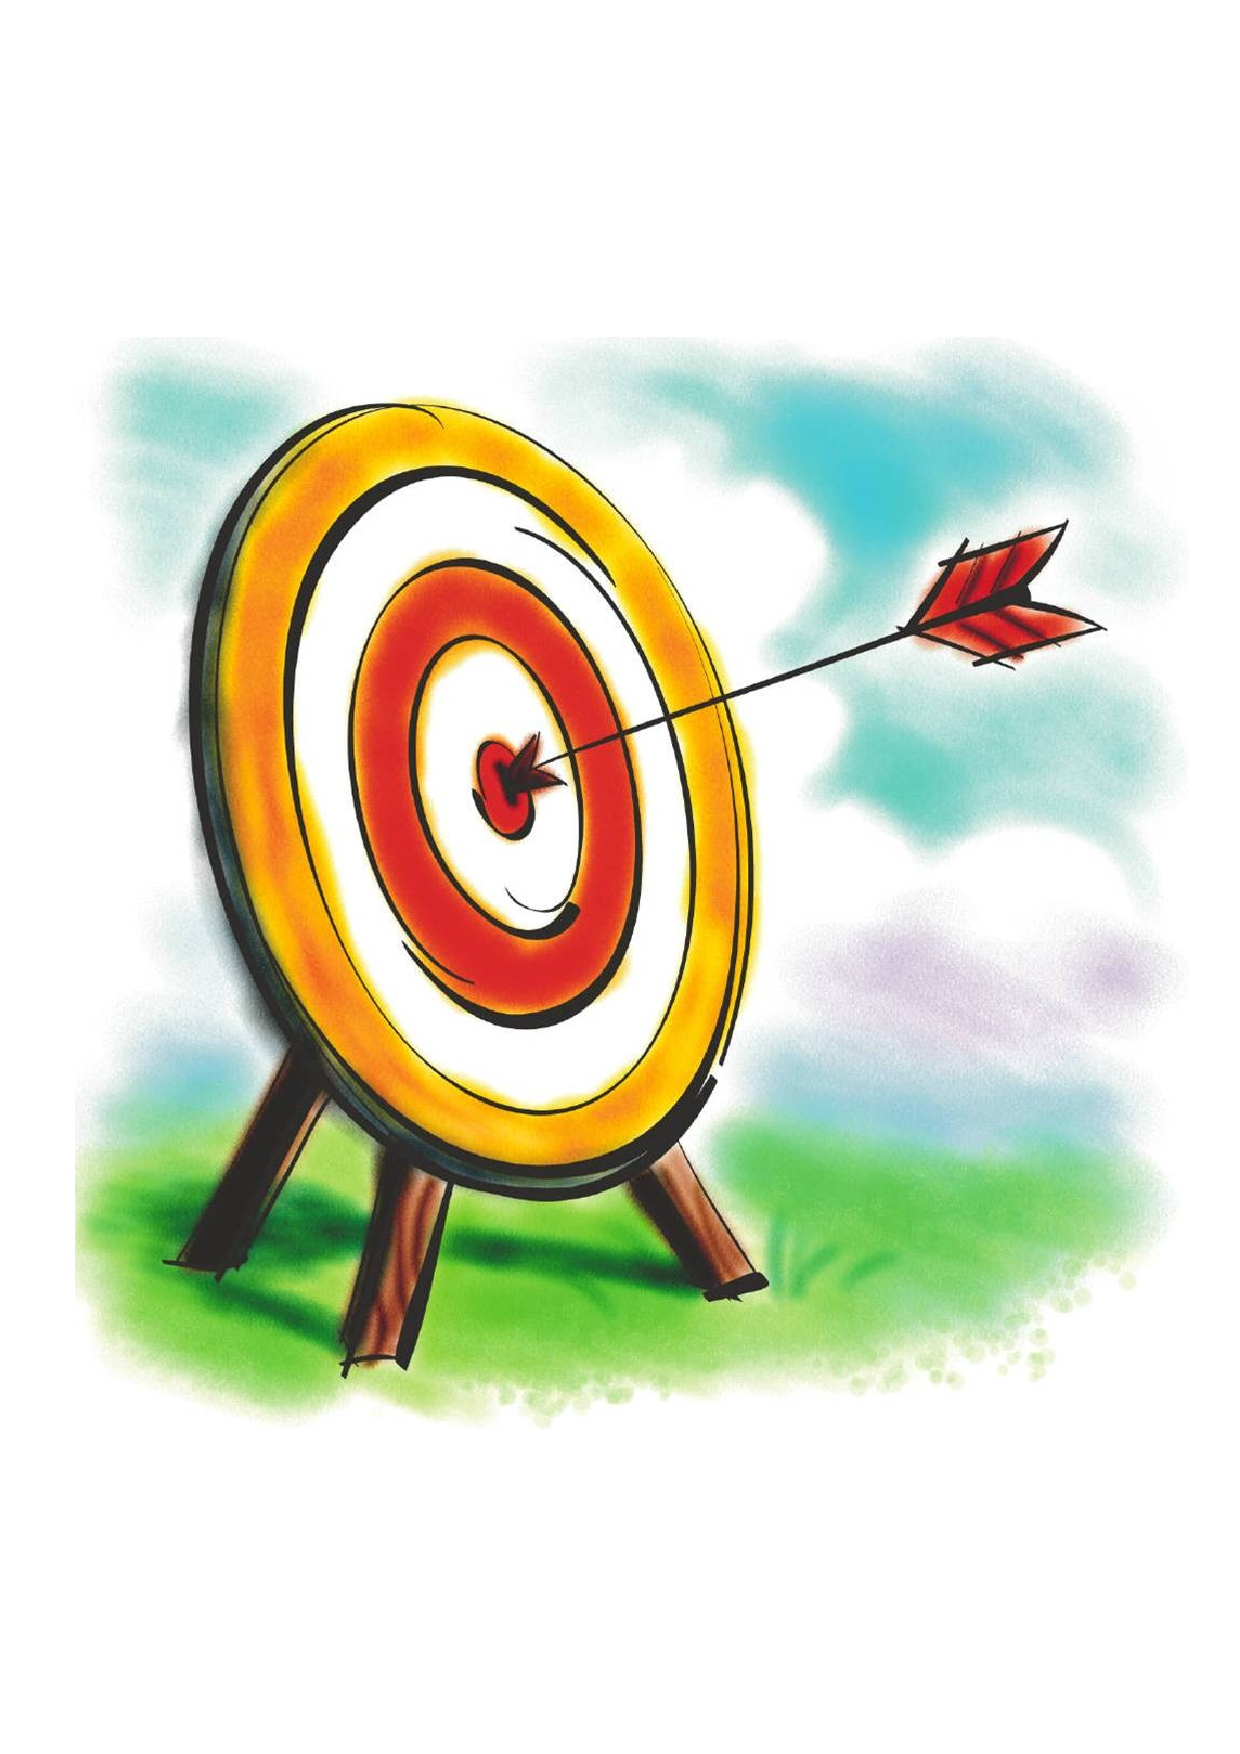
\includegraphics[width=.07\textwidth]{archeryf}}; }
				{\node[fancytitle2,  rounded corners] at (box.west) {\treeBS};}
			}%%
		\end{tikzpicture}
	\end{center}
}%

%%% ============================================================================================

\newcommand{\arcBS}{\noindent\textcolor{red}{\Huge\ding{247}}}
\NewDocumentEnvironment{warning}{g g}{
	\tikzstyle{mybox1} = [draw=red, fill=red!15,very thick, rectangle, rounded corners, inner sep=10pt, inner ysep=20pt]
	\tikzstyle{fancytitle1} =[fill=red!90, text=white]
	\tikzstyle{fancytitle2} =[fill=red!4, text=white]
	\tikzstyle{fancytitle3} =[fill=white, text=white]
	\begin{flushleft}
	\begin{tikzpicture}
	\node [mybox1] (box)\bgroup
	\IfValueTF{#2}{
		\IfFileExists{#2}{\begin{minipage}{.85\textwidth}}{\begin{minipage}{.93\textwidth}}
	}{%%
		\IfFileExists{warining.png}{\begin{minipage}{.85\textwidth}}{\begin{minipage}{.93\textwidth}}
	}%%
	\baselineskip=.95cm
		\begin{RTL}
}{%
		\end{RTL}
	\end{minipage}
	\egroup;
	\IfValueTF{#1}{\node[fancytitle1, left=10pt] at (box.north east) {\hboxR{#1}};}{\node[fancytitle1, left=10pt] at (box.north east) {\hboxR{توجه}};}%
	\IfValueTF{#2}{
		\IfFileExists{#2}
		{\node[fancytitle3, left=3pt,   rounded corners] at (box.west) {\includegraphics[width=.07\textwidth]{#2}}; }
		{\node[fancytitle2,  rounded corners] at (box.west) {\arcBS};}			
	}{%%
		\IfFileExists{warining.png}
		{\node[fancytitle3, left=3pt,   rounded corners] at (box.west) {
\includegraphics[width=.07\textwidth]{warining.png}}; }
		{\node[fancytitle2,  rounded corners] at (box.west) {\arcBS};}
	}%%
	\end{tikzpicture}
	\end{flushleft}
}%

%%% ============================================================================================

\newcommand{\envBS}{\noindent\textcolor{Violet}{\Huge\ding{41}}}
\NewDocumentEnvironment{refer}{g g}{
	\tikzstyle{mybox1} = [draw=Violet, fill=Violet!10,very thick, rectangle, rounded corners, inner sep=10pt, inner ysep=20pt]
	\tikzstyle{fancytitle1} =[fill=Violet!50, text=white]
	\tikzstyle{fancytitle2} =[fill=Violet!20, text=white]
	\tikzstyle{fancytitle3} =[fill=white, text=white]
	\begin{flushleft}
	\begin{tikzpicture}
	\node [mybox1] (box)\bgroup
	\IfValueTF{#2}{
		\IfFileExists{#2}{\begin{minipage}{.85\textwidth}}{\begin{minipage}{.93\textwidth}}
	}{%%
		\IfFileExists{referO.pdf}{\begin{minipage}{.85\textwidth}}{\begin{minipage}{.93\textwidth}}
	}%%
	\baselineskip=.95cm
	\begin{RTL}
}{%
	\end{RTL}
	\end{minipage}
	\egroup;
	\IfValueTF{#1}{\node[fancytitle1, left=10pt] at (box.north east) {\hboxR{#1}};}{\node[fancytitle1, left=10pt] at (box.north east) {\hboxR{مراجع مفید}};}%
	\IfValueTF{#2}{
		\IfFileExists{#2}
		{\node[fancytitle3, left=3pt,   rounded corners] at (box.west) {\includegraphics[width=.07\textwidth]{#2}}; }
		{\node[fancytitle2,  rounded corners] at (box.west) {\envBS};}			
	}{%%
		\IfFileExists{referO.pdf}
		{\node[fancytitle3, left=3pt,   rounded corners] at (box.west) {
\includegraphics[width=.07\textwidth]{referO}}; }
		{\node[fancytitle2,  rounded corners] at (box.west) {\envBS};}
	}%%
	\end{tikzpicture}
	\end{flushleft}
}%

\newcommand{\goodRef}[1]{ \begin{refer} #1 \end{refer} }

%%% ============================================================================================

\newcommand{\twoBS}{\noindent\textcolor{YellowOrange}{\Huge\ding{44}}}
\NewDocumentEnvironment{info}{g g}{
	\tikzstyle{mybox1} = [draw=YellowOrange, fill=YellowOrange!10,very thick, rectangle, rounded corners, inner sep=10pt, inner ysep=20pt]
	\tikzstyle{fancytitle1} =[fill=YellowOrange!50, text=white]
	\tikzstyle{fancytitle2} =[fill=YellowOrange!15, text=white]
	\tikzstyle{fancytitle3} =[fill=white, text=white]
	\begin{flushleft}
	\begin{tikzpicture}
	\node [mybox1] (box)\bgroup
	\IfValueTF{#2}{
		\IfFileExists{#2}{\begin{minipage}{.85\textwidth}}{\begin{minipage}{.93\textwidth}}
	}{
		\IfFileExists{infoRR.png}{\begin{minipage}{.85\textwidth}}{\begin{minipage}{.93\textwidth}}
	}%%
	\baselineskip=.95cm
	\begin{RTL}
}{%
	\end{RTL}
	\end{minipage}
	\egroup;
	\IfValueTF{#1}{\node[fancytitle1, left=10pt] at (box.north east) {\hboxR{#1}};}{\node[fancytitle1, left=10pt] at (box.north east) {\hboxR{مطالب بیشتر}};}%%
	\IfValueTF{#2}{
		\IfFileExists{#2}
		{\node[fancytitle3, left=3pt,   rounded corners] at (box.west) {\includegraphics[width=.07\textwidth]{#2}}; }
		{\node[fancytitle2,  rounded corners] at (box.west) {\twoBS};}			
	}{
		\IfFileExists{infoRR.png}
		{\node[fancytitle3, left=3pt,   rounded corners] at (box.west) {
\includegraphics[width=.07\textwidth]{infoRR}}; }
		{\node[fancytitle2,  rounded corners] at (box.west) {\twoBS};}
	}%%
	\end{tikzpicture}
	\end{flushleft}
}%

%%% ============================================================================================


\newcommand{\teleBS}{\noindent\textcolor{Mulberry}{\Huge\ding{37}}}
\NewDocumentEnvironment{problem}{g g}{
	\tikzstyle{mybox1} = [draw=Mulberry, fill=Mulberry!10,very thick, rectangle, rounded corners, inner sep=10pt, inner ysep=20pt]
	\tikzstyle{fancytitle1} =[fill=Mulberry!50, text=white]
	\tikzstyle{fancytitle2} =[fill=Mulberry!15, text=white]
	\tikzstyle{fancytitle3} =[fill=white, text=white]
	\begin{flushleft}
	\begin{tikzpicture}
	\node [mybox1] (box)\bgroup
	\IfValueTF{#2}{
		\IfFileExists{#2}{\begin{minipage}{.85\textwidth}}{\begin{minipage}{.93\textwidth}}
	}{
		\IfFileExists{home.png}{\begin{minipage}{.85\textwidth}}{\begin{minipage}{.93\textwidth}}
	}%%
	\baselineskip=\baselineskipVar
	\begin{RTL}
}{%
	\end{RTL}
	\end{minipage}
	\egroup;
	\IfValueTF{#1}{\node[fancytitle1, left=10pt] at (box.north east) {\hboxR{#1}};}{\node[fancytitle1, left=10pt] at (box.north east) {\hboxR{سوال}};}%%
	\IfValueTF{#2}{
		\IfFileExists{#2}
		{\node[fancytitle3, left=3pt,   rounded corners] at (box.west) {\includegraphics[width=.07\textwidth]{#2}}; }
		{\node[fancytitle2,  rounded corners] at (box.west) {\twoBS};}			
	}{
		\IfFileExists{home.png}
		{\node[fancytitle3, left=3pt,   rounded corners] at (box.west) {
\includegraphics[width=.07\textwidth]{home}}; }
		{\node[fancytitle2,  rounded corners] at (box.west) {\teleBS};}
	}%%
	\end{tikzpicture}
	\end{flushleft}
}%


%%% =========================================================================================================

\newcommand{\defBS}{\noindent\textcolor{ForestGreen}{\Huge\ding{45}}}
\NewDocumentEnvironment{mydef}{g g}{
	\tikzstyle{mybox1} = [draw=Plum, fill=Plum!15,very thick, rectangle, rounded corners, inner sep=10pt, inner ysep=20pt]
	\tikzstyle{fancytitle1} =[fill=Plum, text=white]
	\tikzstyle{fancytitle2} =[fill=Plum!5, text=white]
	\tikzstyle{fancytitle3} =[fill=white, text=white]
	\begin{center}
		\begin{tikzpicture}
			\node [mybox1] (box)\bgroup
			\IfValueTF{#2}{
				\IfFileExists{#2}{\begin{minipage}{.85\textwidth}}{\begin{minipage}{.93\textwidth}}
			}{%%
				\IfFileExists{defi.png}{\begin{minipage}{.85\textwidth}}{\begin{minipage}{.93\textwidth}}
			}%%
			\baselineskip=.95cm
				\begin{RTL}
}{%
				\end{RTL}
			\end{minipage}
			\egroup;
			\IfValueTF{#1}{\node[fancytitle1, left=10pt] at (box.north east) {\hboxR{#1}};}{\node[fancytitle1, left=10pt] at (box.north east) {\hboxR{تعریف}};}%
			\IfValueTF{#2}{
				\IfFileExists{#2}
				{\node[fancytitle3, left=3pt,   rounded corners] at (box.west) {\includegraphics[width=.07\textwidth]{#2}}; }
				{\node[fancytitle2,  rounded corners] at (box.west) {\defBS};}			
			}{%%
				\IfFileExists{defi.png}
				{\node[fancytitle3, left=3pt,   rounded corners] at (box.west) {
\includegraphics[width=.07\textwidth]{defi}}; }
				{\node[fancytitle2,  rounded corners] at (box.west) {\defBS};}
			}%%
		\end{tikzpicture}
	\end{center}
}%

%%% =========================================================================================================

\newcommand{\commentBSS}{\noindent\textcolor{ForestGreen}{\Huge\ding{23}}}
\NewDocumentEnvironment{mycomment}{g g}{
	\tikzstyle{mybox1} = [draw=red,fill=none,very thick, rectangle, rounded corners, inner sep=10pt, inner ysep=20pt]
	\tikzstyle{fancytitle1} =[fill=red, text=white]
	\tikzstyle{fancytitle2} =[fill=red!5, text=white]
	\tikzstyle{fancytitle3} =[fill=white, text=white]
	\begin{center}
		\begin{tikzpicture}
			\node [mybox1] (box)\bgroup
			\IfValueTF{#2}{
				\IfFileExists{#2}{\begin{minipage}{.85\textwidth}}{\begin{minipage}{.93\textwidth}}
			}{%%
				\IfFileExists{robah.png}{\begin{minipage}{.85\textwidth}}{\begin{minipage}{.93\textwidth}}
			}%%
			\baselineskip=.95cm
				\begin{RTL}
}{%
				\end{RTL}
			\end{minipage}
			\egroup;
			\IfValueTF{#1}{\node[fancytitle1, left=10pt] at (box.north east) {\hboxR{#1}};}{\node[fancytitle1, left=10pt] at (box.north east) {\hboxR{توضیح}};}%
			\IfValueTF{#2}{
				\IfFileExists{#2}
				{\node[fancytitle3, left=3pt,   rounded corners] at (box.west) {\includegraphics[width=.07\textwidth]{#2}}; }
				{\node[fancytitle2,  rounded corners] at (box.west) {\commentBSS};}			
			}{%%
				\IfFileExists{robah.png}
				{\node[fancytitle3, left=3pt,   rounded corners] at (box.west) {
\includegraphics[width=.07\textwidth]{robah}}; }
				{\node[fancytitle2,  rounded corners] at (box.west) {\commentBSS};}
			}%%
		\end{tikzpicture}
	\end{center}
}%

%%% =========================================================================================================



\newtheoremstyle{ntdefinitionstyle}% name of the style to be used
  {\topsep}% measure of space to leave above the theorem. E.g.: 3pt
  {\topsep}% measure of space to leave below the theorem. E.g.: 3pt
  {}% name of font to use in the body of the theorem
  {0pt}% measure of space to indent
  {\bfseries\color{nttitle}}% name of head font
  {}% punctuation between head and body
  {.5em}% space after theorem head; " " = normal interword space
  {}% Manually specify head  

\newtheoremstyle{nttheoremstyle}% name of the style to be used
  {\topsep}% measure of space to leave above the theorem. E.g.: 3pt
  {\topsep}% measure of space to leave below the theorem. E.g.: 3pt
  {}% name of font to use in the body of the theorem
  {0pt}% measure of space to indent
  {\bfseries\color{nttitle}}% name of head font
  {}% punctuation between head and body
  {.2em}% space after theorem head; " " = normal interword space
  {}% Manually specify head
  
\newtheoremstyle{ntplainstyle}% name of the style to be used
  {\topsep}% measure of space to leave above the theorem. E.g.: 3pt
  {\topsep}% measure of space to leave below the theorem. E.g.: 3pt
  {\itshape}% name of font to use in the body of the theorem
  {0pt}% measure of space to indent
  {\bfseries\color{nttitle}}% name of head font
  {}% punctuation between head and body
  {.5em}% space after theorem head; " " = normal interword space
  {}% Manually specify head  



\definecolor{nttitle}{RGB}{0,177,235}
% رنگ آبی کم‌رنگ پس‌زمینه محیط قضیه و محیط lstlisting
\definecolor{ntback}{RGB}{212,237,255}
% رنگ سبز صفحه عنوان فارسی و انگلیسی کتاب، قسمت‌ها و محیط ntpoint
\definecolor{ntsec}{RGB}{204,233,157}
% رنگ قهوه‌ای محیط تعریف
\definecolor{ntdef}{RGB}{205,0,205}

\definecolor{ntexp}{RGB}{224,110,12}


\mdfdefinestyle{theoremstyle}{%
hidealllines=true,
frametitlerule=false,
innerrightmargin=5pt,
innerleftmargin=5pt,
frametitlerulewidth=0pt,
frametitlefont=\color{white}\large\bfseries,
linewidth=2pt,%
frametitlerule=true,%
frametitlebackgroundcolor=nttitle,
innertopmargin=\topskip,
skipabove=.7\baselineskip,
skipbelow=1.8\baselineskip,
backgroundcolor=nttitle!15,
startinnercode={\baselineskip=.9cm},
startcode={\vspace{.8\topsep}},
splitbottomskip=10pt,
theoremseparator={},
needspace=4\baselineskip
align=center,
}
\mdtheorem[style=theoremstyle]{nttheorem}[theorem]{\hspace*{1pt}قضیه}


\newcounter{ntcounter}
\makeatletter
\renewcommand\thentcounter{\thechapter\@SepMark\arabic{ntcounter}} 
\newenvironment{ntpoint}[1][\empty]{\par\begin{mdframed}[
hidealllines=true,
innertopmargin=9pt,
skipabove=.9\baselineskip,
innermargin=\dimexpr-\marginparwidth-\marginparsep\relax,
innerbottommargin=9pt,
innerrightmargin=5pt,innerleftmargin=5pt,
backgroundcolor=ntsec,
  singleextra={
      \node[
        overlay,
        inner ysep=7pt,
       inner xsep=9pt,
        anchor=east,
       % text width=1.2cm,
       % align=left,
        minimum height=4ex,
        fill=nttitle,
        yshift=-5.2mm,
        xshift=0mm,
        %rounded corners=3pt,
        font=\color{white}\bfseries
      ] at (P) {\rl{نکته~\thentcounter}};
        \draw[white,fill=white] ($(P)-(0pt,1.65mm)$) -- ($(P)-(0pt,8.8mm)$) -- ($(P)-(7pt,5.225mm)$) -- cycle;
      },
   firstextra={
      \node[
       overlay,
        inner ysep=7pt,
       inner xsep=9pt,
        anchor=east,
       % text width=1.2cm,
       % align=left,
        minimum height=4ex,
        fill=nttitle,
        yshift=-5.2mm,
        xshift=0mm,
        %rounded corners=3pt,
        font=\color{white}\bfseries
      ] at (P) {\rl{نکته~\thentcounter}};
        \draw[white,fill=white] ($(P)-(0pt,1.65mm)$) -- ($(P)-(0pt,8.8mm)$) -- ($(P)-(7pt,5.225mm)$) -- cycle;
      },
]\baselineskip=\baselineskipVar\refstepcounter{ntcounter}
\textbf{\ifx\empty#1\hspace*{1.9cm}\relax\else\hspace*{1.65cm}(#1)\fi}%\\[.2cm]%
\noindent\ignorespaces%
\noindent}{\end{mdframed}\par\vspace*{.4ex}}
\@addtoreset{ntcounter}{chapter}
\makeatother


%%%%%%%%%%%%%%%%%%%%%%%%%%%%%%%%%%%%%%%%%%%%%%%%%
% تعریف محیط ntexample


\newcounter{ntexample}
\makeatletter
\renewcommand\thentexample{\thechapter\@SepMark\arabic{ntexample}} 

\newenvironment{ntexample}[1][\empty]{\par\begin{mdframed}[roundcorner=10pt,,align=right,skipabove=.5\baselineskip,
skipbelow=.3\baselineskip,
innertopmargin=10pt,
innerbottommargin=12pt,
usetwoside=false,
innerrightmargin=10pt,
rightmargin=3pt,
innerleftmargin=0pt,
%outermargin=1pt,
%backgroundcolor=brown!25,
 topline=false,bottomline=false,leftline=false,
middlelinewidth=8pt,
%splittopskip=-15pt,
splitbottomskip=5pt,
middlelinecolor=ntexp,
  singleextra={
      \node[
        overlay,
        outer sep=0pt,
        anchor=north west,
        text width=2.1cm,
        minimum height=4ex,
        fill=ntexp,
        yshift=-2mm,
        xshift=-21mm,
        %rounded corners=3pt,
        font=\color{white}\bfseries
      ] at (P) {\rl{مثال~\thentexample}};
      },
   firstextra={
      \node[
        overlay,
        outer sep=0pt,
        anchor=north west,
        text width=2.1cm,
        minimum height=4ex, 
        fill=ntexp,
        yshift=-2mm,
        xshift=-21mm,
        %rounded corners=3pt,
        font=\color{white}\bfseries
      ] at (P) {\rl{مثال~\thentexample}};
      },
]
\baselineskip=\baselineskipVar
\refstepcounter{ntexample}
\hspace*{1.8cm}\textbf{\ifx\empty#1\space\relax\else\space\textcolor{nttitle}{#1}\space \ \fi}%\\[.2cm]%
%\noindent\ignorespaces%
}{\end{mdframed}\par}
\@addtoreset{ntexample}{chapter}
\makeatother


\newenvironment{ntexample2}[1][\empty]{\par\begin{mdframed}[roundcorner=10pt,,align=right,skipabove=.5\baselineskip,
skipbelow=.3\baselineskip,
innertopmargin=10pt,
innerbottommargin=12pt,
usetwoside=false,
innerrightmargin=10pt,
rightmargin=3pt,
innerleftmargin=0pt,
%outermargin=1pt,
%backgroundcolor=brown!25,
 topline=false,bottomline=false,leftline=false,
middlelinewidth=8pt,
%splittopskip=-15pt,
splitbottomskip=5pt,
middlelinecolor=ntexp,
  singleextra={
      \node[
        overlay,
        outer sep=0pt,
        anchor=north west,
        text width=2.1cm,
        minimum height=4ex,
        fill=ntexp,
        yshift=-2mm,
        xshift=-21mm,
        %rounded corners=3pt,
        font=\color{white}\bfseries
      ] at (P) {\rl{مثال}};
      },
   firstextra={
      \node[
        overlay,
        outer sep=0pt,
        anchor=north west,
        text width=2.1cm,
        minimum height=4ex, 
        fill=ntexp,
        yshift=-2mm,
        xshift=-21mm,
        %rounded corners=3pt,
        font=\color{white}\bfseries
      ] at (P) {\rl{مثال}};
      },
]
\baselineskip=\baselineskipVar
\hspace*{1.8cm}\textbf{\ifx\empty#1\space\relax\else\space\textcolor{nttitle}{#1}\space \ \fi}%\\[.2cm]%
%\noindent\ignorespaces%
}{\end{mdframed}\par}
\makeatother

\makeatletter
\newenvironment{ntremember}[1][\empty]{\par\begin{mdframed}[roundcorner=10pt,,align=right,skipabove=.5\baselineskip,
skipbelow=.3\baselineskip,
innertopmargin=10pt,
innerbottommargin=12pt,
usetwoside=false,
innerrightmargin=10pt,
rightmargin=3pt,
innerleftmargin=0pt,
%outermargin=1pt,
%backgroundcolor=brown!25,
 topline=false,bottomline=false,leftline=false,
middlelinewidth=8pt,
%splittopskip=-15pt,
splitbottomskip=5pt,
middlelinecolor=ForestGreen,
  singleextra={
      \node[
        overlay,
        outer sep=0pt,
        anchor=north west,
        text width=2.1cm,
        minimum height=4ex,
        fill=ForestGreen,
        yshift=-2mm,
        xshift=-21mm,
        %rounded corners=3pt,
        font=\color{white}\bfseries
      ] at (P) {\rl{یادآوری}};
      },
   firstextra={
      \node[
        overlay,
        outer sep=0pt,
        anchor=north west,
        text width=2.1cm,
        minimum height=4ex, 
        fill=ForestGreen,
        yshift=-2mm,
        xshift=-21mm,
        %rounded corners=3pt,
        font=\color{white}\bfseries
      ] at (P) {\rl{یادآوری}};
      },
]
\baselineskip=\baselineskipVar
\hspace*{1.8cm}\textbf{\ifx\empty#1\space\relax\else\space\textcolor{nttitle}{#1}\space \ \fi}%\\[.2cm]%
%\noindent\ignorespaces%
}{\end{mdframed}\par}
\makeatother


\newenvironment{ntdefinition}[1][\empty]{\par\begin{mdframed}[roundcorner=10pt,,align=right,skipabove=.5\baselineskip,
skipbelow=.5\baselineskip,
innertopmargin=10pt,
innerbottommargin=0pt,
usetwoside=false,
innerrightmargin=10pt,
rightmargin=3pt,
innerleftmargin=0pt,
%outermargin=1pt,
%backgroundcolor=brown!25,
 topline=false,bottomline=false,leftline=false,
middlelinewidth=8pt,
%splittopskip=-15pt,
splitbottomskip=5pt,
middlelinecolor=ntdef,
  singleextra={
      \node[
        overlay,
        outer sep=0pt,
        anchor=north west,
        text width=2.1cm,
        minimum height=4ex,
        fill=ntdef,
        yshift=-2mm,
        xshift=-21mm,
        %rounded corners=3pt,
        font=\color{white}\bfseries
      ]     at (P) {\rl{تعریف~\thedefinition}};
      },
   firstextra={
      \node[
        overlay,
        outer sep=0pt,
        anchor=north west,
        text width=2.1cm,
        minimum height=4ex, 
        fill=ntdef,
        yshift=-2mm,
        xshift=-21mm,
        %rounded corners=3pt,
        font=\color{white}\bfseries
      ] at (P) {\rl{تعریف~\thedefinition}};
      },
]
\baselineskip=\baselineskipVar
\refstepcounter{definition}
\hspace*{1.8cm}\textbf{\ifx\empty#1\space\relax\else\space\textcolor{nttitle}{#1}\space \ \fi}%
%\noindent\ignorespaces%
}{\end{mdframed}\hspace*{1.5cm} \par}

%%%%%%%%%%%%%%%%%%%%%%%%%%%%%%%%%%%%%%%%%%%%%%%%%
% تعریف محیط ntsolution
\newenvironment{ntsolution}{\par\begin{mdframed}[skipabove=.7\baselineskip,
innertopmargin=0pt,
innerbottommargin=0pt,
innerrightmargin=8pt,innerleftmargin=0pt,
outermargin=-1pt,
%backgroundcolor=green,
 topline=false,bottomline=false,leftline=false,
middlelinewidth=8pt,
middlelinecolor=nttitle,
]
\baselineskip=\baselineskipVar
\textbf{\textcolor{nttitle}{حل}}\ \
\noindent}{\end{mdframed}\par}

%%%%%%%%%%%%%%%%%%%%%%%%%%%%%%%%%%%%%%%%%%%%%%%%%
% تعریف محیط ntproblems برای حروف‌چینی تمرین‌های پایان فصل‌ها
\makeatletter
\newenvironment{ntproblems}[1][تمرین‌ها]{%
\renewcommand{\thesection}{}
\phantomsection\addcontentsline{toc}{section}{\hspace*{2pt}#1}
\vspace*{.7\baselineskip}
\needspace{5\baselineskip}
\begin{fullwidth}
\par
\begin{mdframed}[%outermargin=\dimexpr-\marginparwidth-\marginparsep\relax,align=center,%skipabove=.7\baselineskip,
%skipbelow=.1\baselineskip,
innertopmargin=9pt,
innerbottommargin=9pt,
%outermargin=-5pt,
usetwoside=false,
rightmargin=0pt,
innerrightmargin=5pt,innerleftmargin=0pt,
backgroundcolor=nttitle!15,
topline=false,
bottomline=false,leftline=false,
middlelinewidth=20pt,
middlelinecolor=nttitle,
]
\normalfont\Large\bfseries #1
\end{mdframed}%
\end{fullwidth}
\vspace*{-.5\baselineskip}
\sectionmark{#1}
\renewcommand\theenumi{\color{nttitle}\bfseries\thechapter\@SepMark\arabic{enumi}}
\renewcommand\labelenumi{\theenumi}
\let\p@enumii\@empty
\setlength{\columnsep}{5ex}
\begin{adjmulticols*}{2}{-\dimexpr+\marginparwidth+\marginparsep\relax}{}
\begin{enumerate}[align=left,itemindent=0pt,labelwidth=5ex,leftmargin=6ex
]}
{\end{enumerate}
\raggedcolumns
\end{adjmulticols*}
}  
\makeatother

%%%%%%%%%%%%%%%%%%%%%%%%%%%%%%%%%%%%%%%%%%%%%%%%%
% تعریف محیط ntsolutions برای حروف‌چینی پاسخ تمرین‌ها
\newenvironment{ntsolutions}{%
\setlength{\columnsep}{5ex}
\begin{adjmulticols*}{2}{-\dimexpr+\marginparwidth+\marginparsep\relax}{}
}
{
\raggedcolumns
\end{adjmulticols*}
}  

%%%%%%%%%%%%%%%%%%%%%%%%%%%%%%%%%%%%%%%%%%%%%%%%%
% تعریف دستور ntchsol برای مشخص کردن پاسخ‌های مربوط به هر فصل در محیط ntsolutions
\newcommand{\ntchsol}[1]{
%\vspace*{.7\baselineskip}
%\needspace{4\baselineskip}
\par
\begin{mdframed}[%outermargin=\dimexpr-\marginparwidth-\marginparsep\relax,align=center,
skipabove=.7\baselineskip,
%skipbelow=.1\baselineskip,
innertopmargin=9pt,
innerbottommargin=9pt,
%outermargin=-5pt,
usetwoside=false,
rightmargin=0pt,
innerrightmargin=5pt,innerleftmargin=0pt,
backgroundcolor=nttitle!15,
topline=false,
bottomline=false,leftline=false,
middlelinewidth=20pt,
middlelinecolor=nttitle,
]
\normalfont\Large\bfseries #1
\end{mdframed}%
%\end{fullwidth}
\vspace*{-.5\baselineskip}
}

%%%%%%%%%%%%%%%%%%%%%%%%%%%%%%%%%%%%%%%%%%%%%%%%%

\def\lemmaautorefname{لم}










